\chapter{Messtechnik und Systemarchitektur}
\label{ch:messtechnik}

Um eine fundierte Analyse des Kühlsystems durchzuführen und die theoretischen Modelle zu validieren, ist eine präzise und hochfrequente Datenerfassung unerlässlich. Dieses Kapitel beschreibt die messtechnische Infrastruktur des Fahrzeugs sowie die zugrunde liegende Systemarchitektur. Dabei wird zunächst auf die bereits im Fahrzeug integrierte Bestandssensorik eingegangen, bevor die im Rahmen dieser Arbeit implementierten Erweiterungen zur detaillierten thermischen Überwachung erläutert werden. Ziel ist es, eine lückenlose Messkette abzubilden – von der physikalischen Messgröße über die Signalaufbereitung bis hin zur digitalen Protokollierung im Datenlogger.

\section{Bestandssensorik und Infrastruktur}
\label{sec:bestandssensorik}

Die am Fahrzeug vorhandene elektronische Infrastruktur bildet das Rückgrat der Datenerfassung und Steuerung, auf dem die thermische Analyse dieser Arbeit aufbaut. Ein tiefgreifendes Verständnis der vorhandenen Signalwege ist essenziell, um die Qualität und Aussagekraft der geloggten Daten korrekt einordnen zu können.

\begin{figure}[htbp]
    \centering
    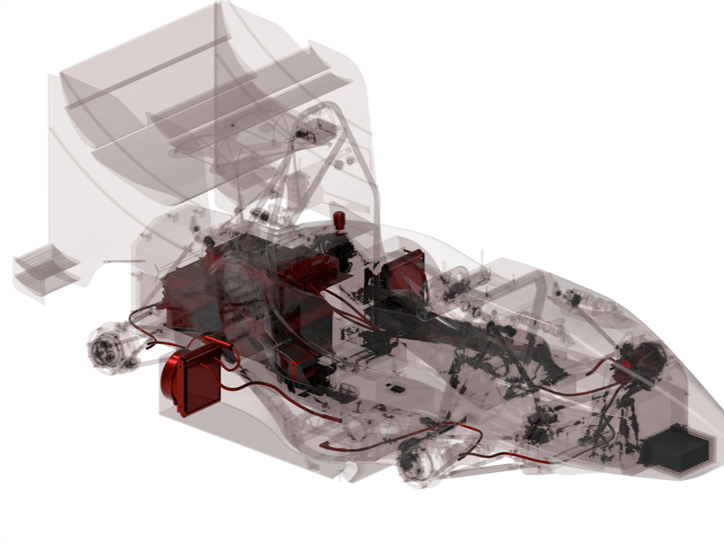
\includegraphics[width=0.9\textwidth]{pics/Systemarchtiektur_RP25e.png}
    \caption{Schematische Übersicht der fahrzeugseitigen Systemarchitektur: Signalfluss von den Sensoren über VCU und PDU bis zum Datenlogger.}
    \label{fig:Systemarchtiektur_RP25e}
\end{figure}

\subsection{Zentrale Steuereinheiten (VCU \& PDU)}
\label{subsec:vcu_pdu}

Die Steuerung und Energieversorgung des Fahrzeugs wird durch zwei zentrale Einheiten realisiert, die maßgeblich an der Datenerhebung für das Kühlsystem beteiligt sind.

\paragraph{Vehicle Control Unit (VCU)}
Die VCU stellt das Herzstück der Fahrzeugsteuerung dar. Auf ihr wird die Steuerungssoftware ausgeführt, welche die gesamte Betriebsstrategie verwaltet. Im Kontext des Kühlsystems übernimmt die VCU zwei Hauptaufgaben:
\begin{enumerate}
    \item \textbf{Aktorik-Ansteuerung:} Basierend auf definierten Temperaturschwellwerten regelt die VCU die Drehzahl der Kühlmittelpumpen und die Aktivierung der Lüfter über ein PWM-Signal.
    \item \textbf{Daten-Gateway:} Sie fungiert als zentraler Knotenpunkt, der Messwerte der Inverter via CAN-Bus sowie analoge Sensordaten empfängt, verarbeitet und an den Datenlogger weiterleitet.
\end{enumerate}

Eine Limitierung der VCU besteht darin, dass viele physikalische Sensoren aufgrund geringer Signalstärken oder hoher Ausgangsimpedanzen nicht direkt angeschlossen werden können. Diese erfordern eine vorgeschaltete Signalaufbereitung, was die Anzahl der direkt nutzbaren Sensoreingänge effektiv begrenzt.

\begin{figure}[htbp]
    \centering
    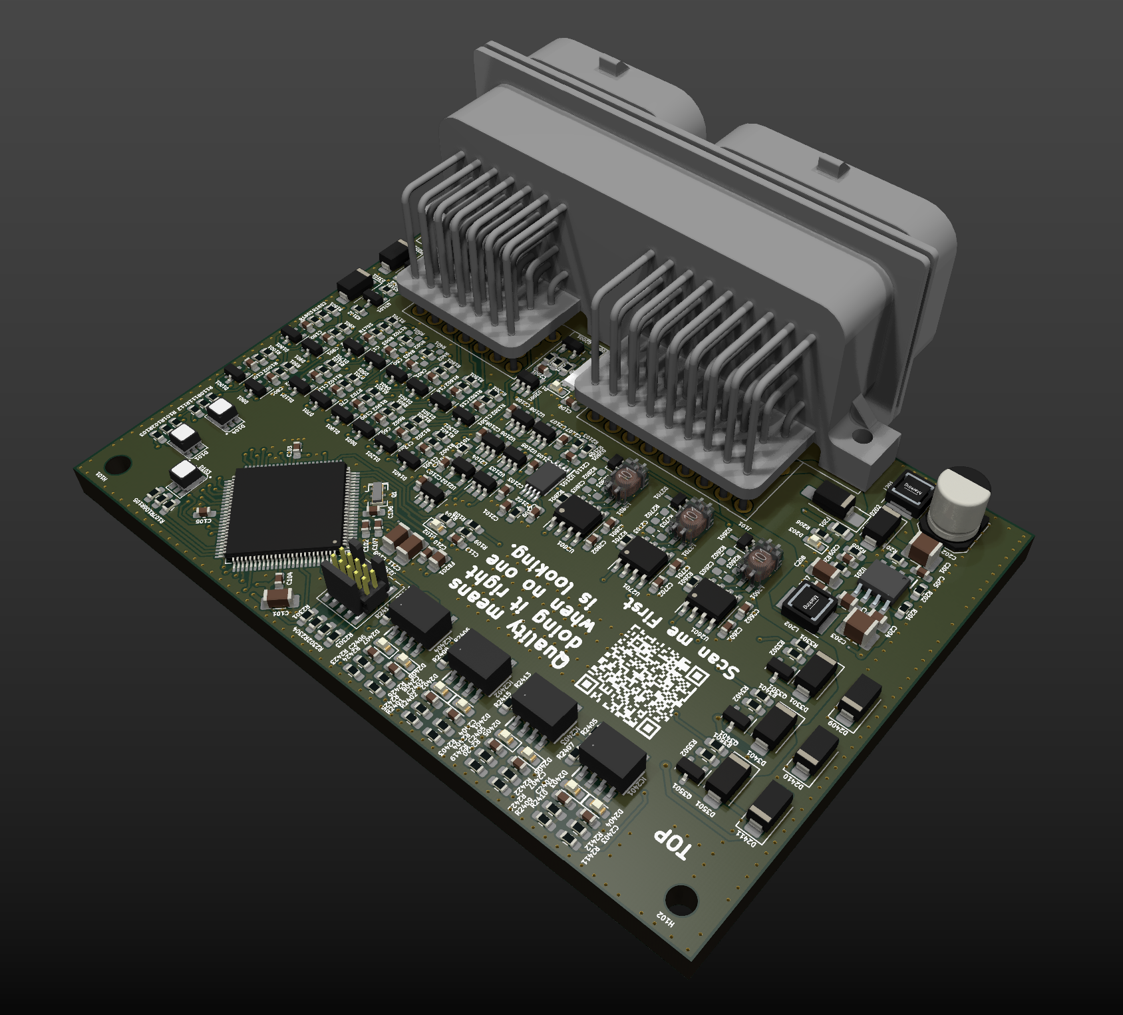
\includegraphics[width=0.7\textwidth]{pics/VCU_PCB.png}
    \caption{Übersicht der VCU}
    \label{fig:vcu_uebersicht}
\end{figure}


\paragraph{Power Distribution Unit (PDU)}
Die PDU fungiert als intelligente, softwarebasierte Stromverteilung und ersetzt klassische Schmelzsicherungen durch elektronisch überwachte Kanäle. Ihre Relevanz für die Messtechnik liegt in der kontinuierlichen Stromüberwachung der angeschlossenen Aktoren:
\begin{itemize}
    \item \textbf{Lastüberwachung:} Die PDU misst die Stromaufnahme der Kühlmittelpumpen und Lüfter. Diese Daten erlauben Rückschlüsse auf den Betriebszustand der Aktorik, beispielsweise bei Blockaden oder Trockenlauf.
    \item \textbf{Versorgungsstabilität:} Durch das Monitoring der Bordnetzspannung wird sichergestellt, dass die Sensorik stets innerhalb ihrer spezifizierten Versorgungsspannung arbeitet, was die Validität der Messergebnisse absichert.
\end{itemize}

\begin{figure}[htbp]
    \centering
    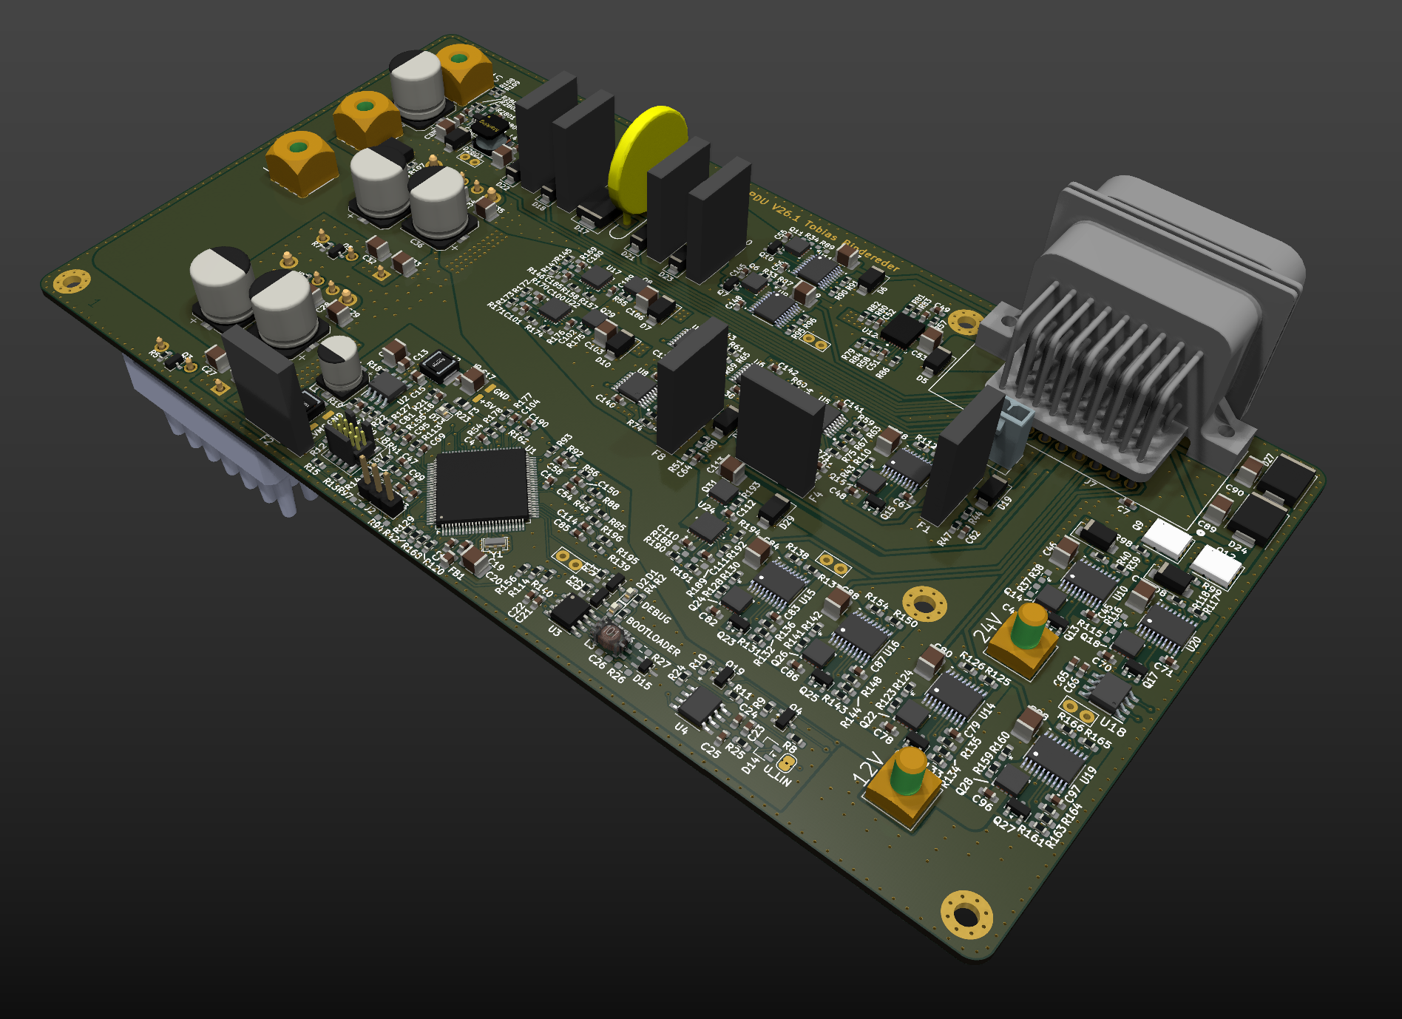
\includegraphics[width=0.7\textwidth]{pics/PDU_PCB.png}
    \caption{Übersicht der PDU}
    \label{fig:PDU_uebersicht}
\end{figure}

Zusammen bilden VCU und PDU die Grundlage, um nicht nur Temperaturen, sondern auch die dafür aufgewendete elektrische Energie und den Betriebszustand der Aktoren zu protokollieren.

\subsection{Datenerfassung und Telemetrie}
\label{subsec:datenlogger}

Die zentrale Einheit zur persistenten Speicherung aller fahrzeugrelevanten Daten ist der Datenlogger. Er erfasst kontinuierlich die von der VCU sowie den Invertern via CAN-Bus bereitgestellten Messwerte und speichert diese mit hoher Abtastrate auf einem internen Speichermedium.

\begin{figure}[htbp]
    \centering
    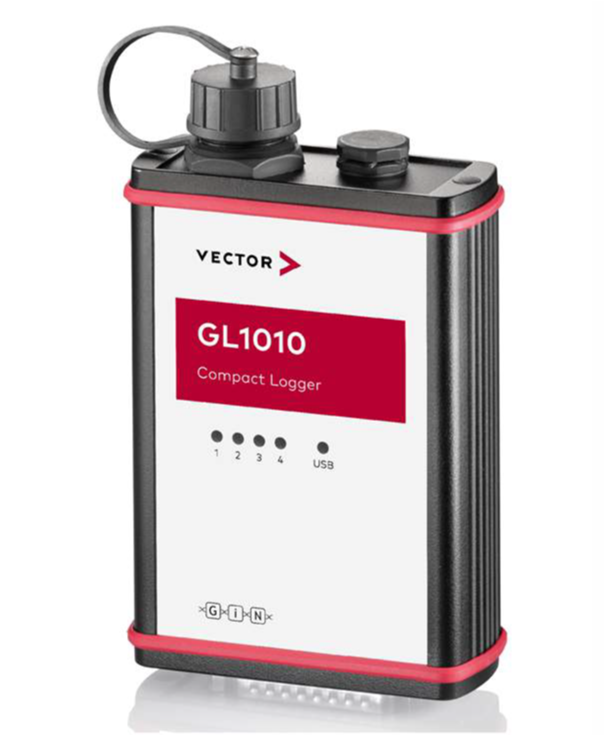
\includegraphics[width=0.7\textwidth]{pics/Vector Logger GL1010.png}
    \caption{Verbauter Vector Logger GL1010 mit CAN-Bus-Anbindung und Speichermedium.}
    \label{fig:datenlogger}
\end{figure}

Zur Auswertung der umfangreichen Datensätze wird ein eigens entwickeltes MATLAB-Skript eingesetzt. Dieses ermöglicht es, die Rohdaten zu filtern, physikalische Einheiten zuzuordnen und thermische Zusammenhänge -- wie etwa die Trägheit des Kühlmittels im Verhältnis zu Lastspitzen der Motoren -- zu visualisieren. Erst durch diese automatisierte Aufbereitung lassen sich die im Wettbewerb oder auf dem Prüfstand gewonnenen Daten für die Validierung der Kühlungsauslegung nutzen.

\subsection{Signalaufbereitung mittels Messbrücken}
\label{subsec:messbruecken}

Da viele physikalische Sensoren -- insbesondere piezoresistive Druckaufnehmer -- auf minimalen Widerstandsänderungen basieren, ist eine direkte Auswertung durch die Analogeingänge der VCU aufgrund des geringen Signal-Rausch-Verhältnisses nicht zielführend. Zur Wandlung dieser Differenzen in ein nutzbares Spannungssignal wird die Wheatstone-Brückenschaltung eingesetzt.

\begin{figure}[htbp]
    \centering
    % \includegraphics[width=0.55\textwidth]{pics/wheatstone_bridge.png}
    \caption{Schaltplan einer Wheatstone-Brückenschaltung zur Wandlung von Widerstandsänderungen in eine proportionale Messspannung $\Delta U$.}
    \label{fig:wheatstone_bridge}
\end{figure}

Ein wesentlicher Vorteil dieses differenziellen Messprinzips ist die Kompensation von Störeinflüssen:
\begin{itemize}
    \item \textbf{Temperaturkompensation:} Da sich Leitungswiderstände bei Erwärmung in allen Brückenzweigen ähnlich ändern, heben sich diese Fehler gegenseitig auf.
    \item \textbf{Nullpunktstabilität:} Die Brücke erlaubt eine hohe Auflösung um den Arbeitspunkt, was besonders bei der Detektion feiner Druckunterschiede im Kühlkreislauf essenziell ist.
\end{itemize}

Die Anzahl der verfügbaren Messbrücken ist durch den Bauraum und die Komplexität der Signalverstärkung begrenzt, weshalb eine gezielte Priorisierung der thermisch kritischsten Messstellen erforderlich ist.

\section{Sensorik der Antriebseinheiten}
\label{sec:antriebssensorik}

\paragraph{Temperaturüberwachung der Antriebsmotoren}
\label{sec:motor}

Jeder Antriebsmotor verfügt über einen in die Statorwicklung eingebetteten PT1000-Widerstandsthermometer. Dieser misst die Wicklungstemperatur direkt an der thermisch kritischsten Stelle des Motors. Das physikalische Messprinzip wird in Abschnitt~\ref{subsec:pt1000} detailliert beschrieben, da es identisch mit den zusätzlich verbauten Kühlmitteltemperatursensoren ist.

\begin{figure}[htbp]
    \centering
    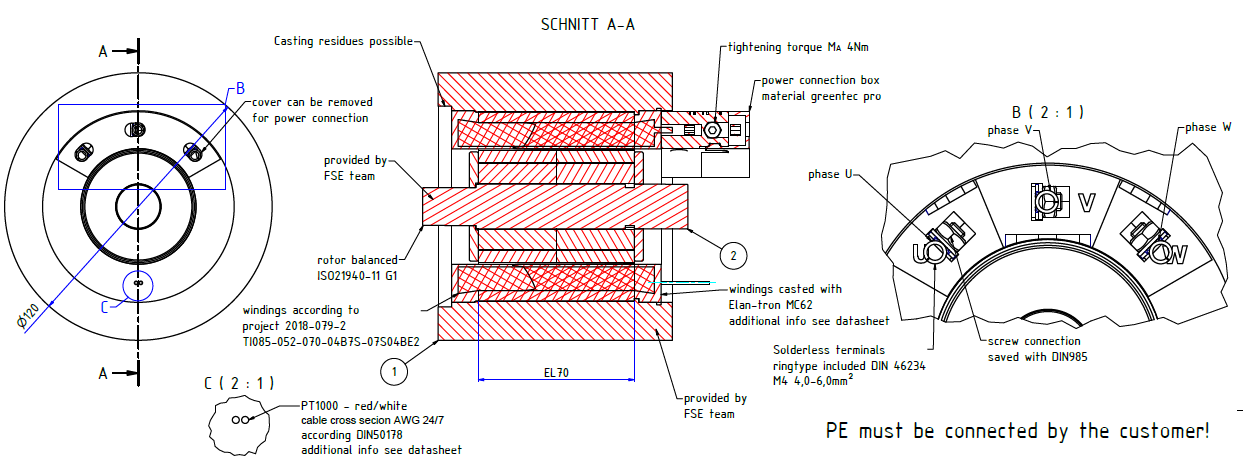
\includegraphics[width=0.7\textwidth]{pics/Motor_Data_sheet.PNG}
    \caption{Einbaulage des PT1000-Sensors in der Statorwicklung eines Antriebsmotors.}
    \label{fig:motor_pt1000}
\end{figure}

\paragraph{Integrierte Sensorik der Inverter}

Jeder Inverter verfügt über einen im IGBT-Modul (Insulated Gate Bipolar Transistor) integrierten Temperatursensor. Dieser erlaubt die direkte Abfrage der Sperrschichttemperatur der Leistungshalbleiter, welche als kritische Betriebsgröße kontinuierlich mitgeloggt wird. Da der Inverterhersteller die Veröffentlichung von Produktabbildungen nicht gestattet, zeigt Abbildung~\ref{fig:inverter_igbt} exemplarisch einen Inverter eines Wettbewerbers, der ein vergleichbares Kühlungskonzept realisiert.

\begin{figure}[htbp]
    \centering
    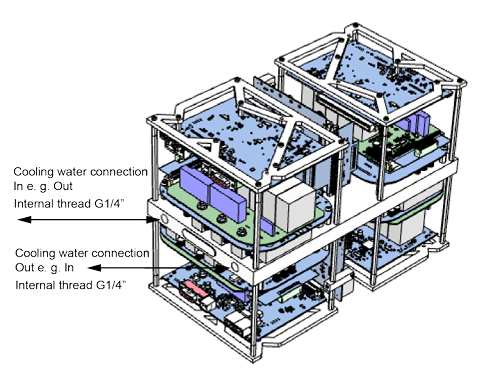
\includegraphics[width=0.7\textwidth]{pics/AMK_Inverter.PNG}
    \caption{Exemplarische Darstellung eines IGBT-Invertermoduls mit integriertem Temperatursensor (Fremdprodukt, da Herstellerfreigabe nicht vorliegt). Das Kühlungskonzept ist vergleichbar mit dem eingesetzten System.}
    \label{fig:inverter_igbt}
\end{figure}

\paragraph{Kühlmittelpumpen und PWM-Ansteuerung}

Im Fahrzeug sind zwei Kühlmittelpumpen verbaut, die die beiden Kühlkreisläufe -- Motorkreislauf und Inverterkreislauf -- unabhängig voneinander versorgen. Die Pumpen ermöglichen keine direkte Messung des Volumenstroms, und eine separate Stromerfassung je Pumpe ist im aktuellen Systemaufbau nicht vorgesehen. Dennoch wird das PWM-Ansteuersignal, das die VCU an die Pumpen sendet, mitgeloggt. Dies erlaubt eine qualitative Nachvollziehbarkeit des Pumpenbetriebszustands in der Datenanalyse. Die fehlende Volumenstromerfassung stellt jedoch eine wesentliche Messlücke dar, die im Rahmen dieser Arbeit durch einen zusätzlichen Durchflusssensor geschlossen wird (siehe Abschnitt~\ref{subsec:volumenstrom}).

\begin{figure}[htbp]
    \centering
    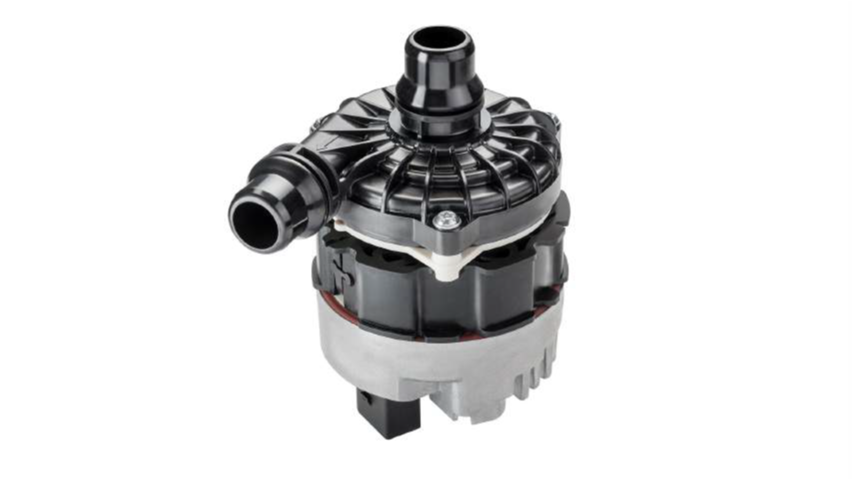
\includegraphics[width=0.7\textwidth]{pics/Pumpe_Vitesco.png}
    \caption{Verbaute Pumpe der Firma Vitesco mit 24V und (60W) Leistung.}
    \label{fig:pumpen_einbau}
\end{figure}

\section{Projektspezifische Erweiterung der Messtechnik}
\label{sec:erweiterung}

Die in Abschnitt~\ref{sec:bestandssensorik} beschriebene Bestandssensorik liefert zwar eine solide Ausgangsbasis, lässt jedoch für eine vollständige thermische Bilanzierung des Kühlsystems wesentliche Messgrößen offen. Im Rahmen dieser Arbeit wird die Messtechnik daher gezielt um zwei Sensortypen erweitert: einen Volumenstromsensor sowie zusätzliche Temperaturmessstellen

\subsection{Volumenstrom-Sensor}
\label{subsec:volumenstrom}

Zur präzisen Bestimmung des Volumenstroms -- und damit zur Berechnung des Massenstroms, der für die thermische Leistungsbilanz des Kühlkreislaufs essenziell ist -- wird ein Turbinen-Durchflusssensor eingesetzt. Abbildung~\ref{fig:durchfluss_sensor_foto} zeigt den verbauten Sensor, Abbildung~\ref{fig:durchfluss_sensor_prinzip} erläutert das zugrunde liegende Wirkprinzip.

\begin{figure}[htbp]
    \centering
    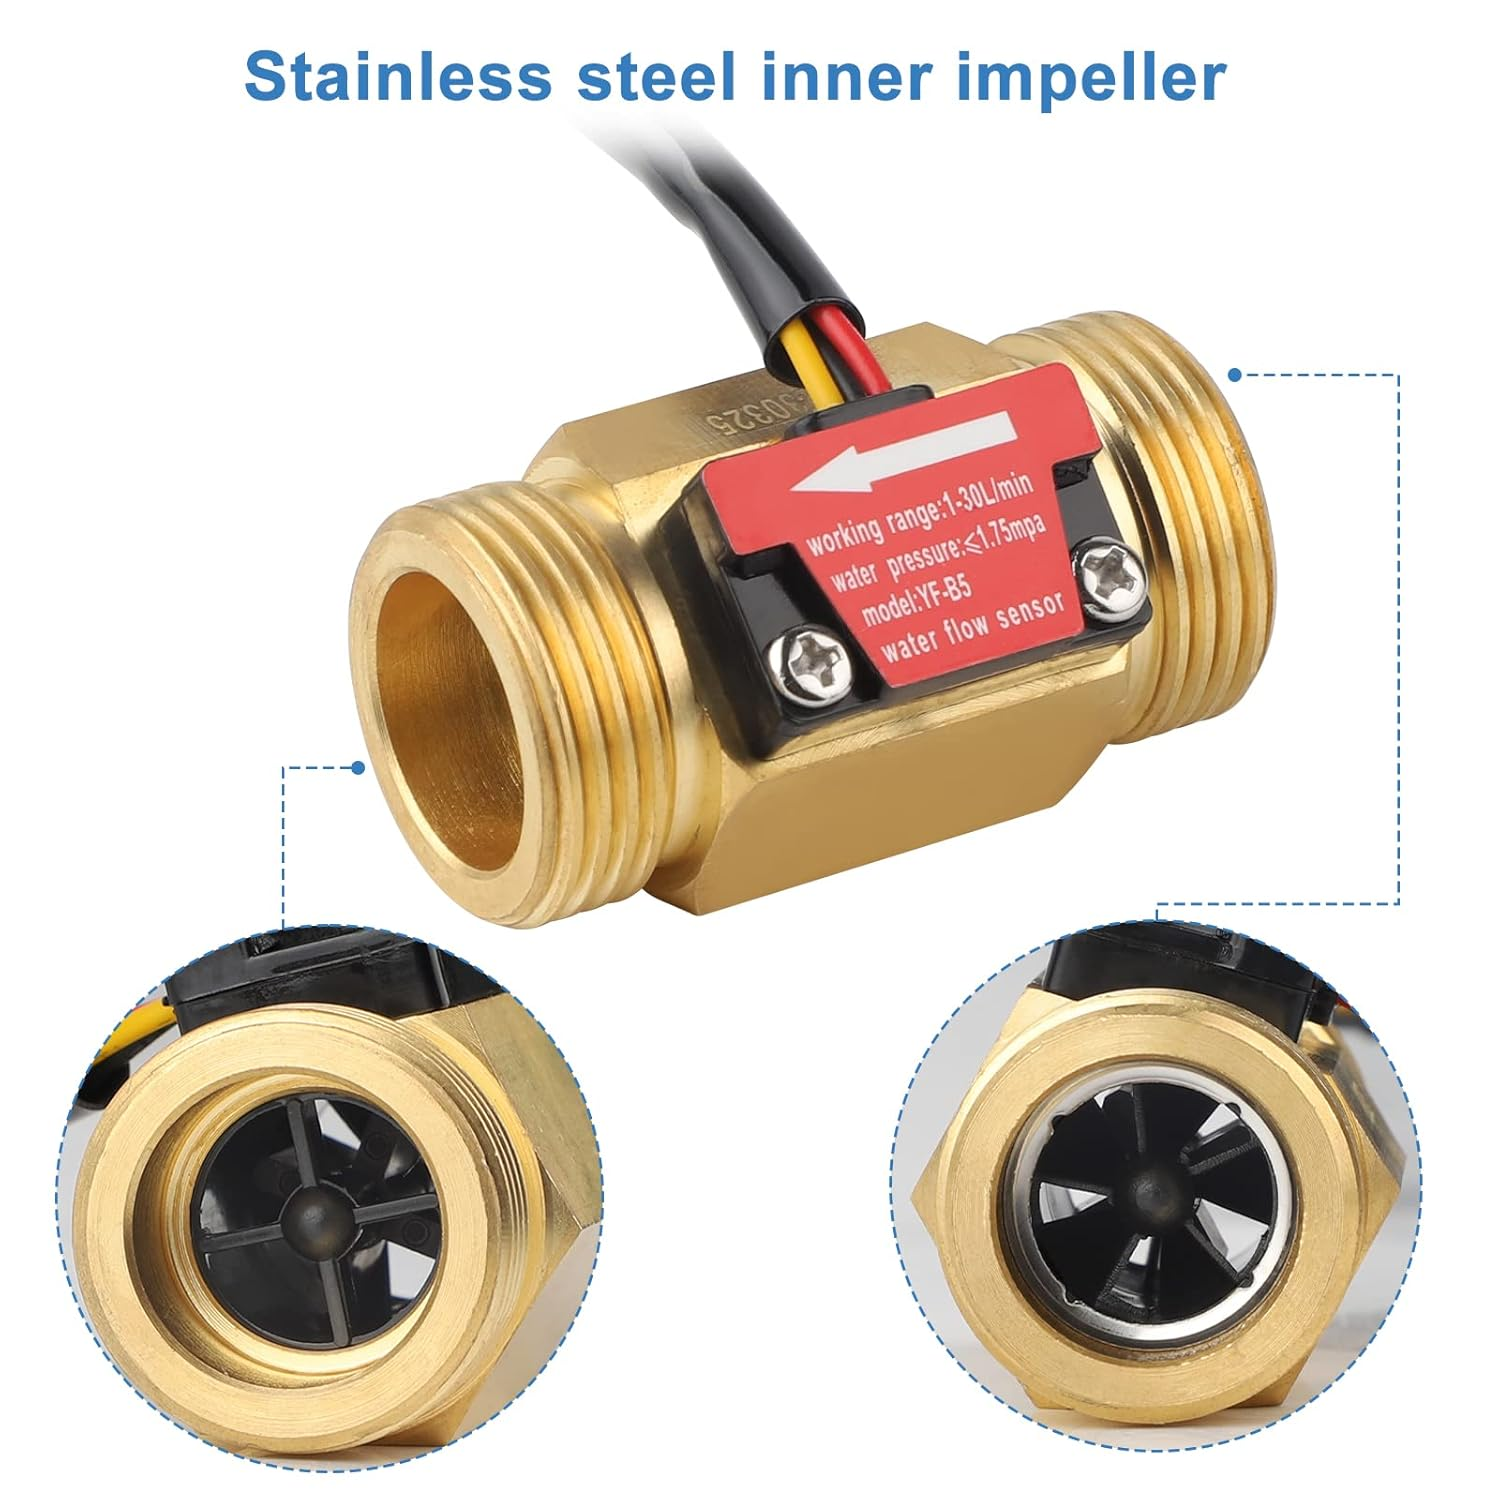
\includegraphics[width=0.6\textwidth]{pics/Volumenstrom_Sensor_neu.jpg}
    \caption{Verbauter Turbinen-Durchflusssensor im Kühlkreislauf des Fahrzeugs.}
    \label{fig:durchfluss_sensor_foto}
\end{figure}

Das Funktionsprinzip basiert auf der Wandlung der Strömungsenergie in eine Rotationsbewegung. Die einströmende Kühlflüssigkeit wird durch Leitschaufeln stabilisiert und auf den Rotor geleitet, dessen Winkelgeschwindigkeit über einen weiten Messbereich linear proportional zur mittleren Strömungsgeschwindigkeit ist. Ein im Rotor integrierter Permanentmagnet erzeugt bei jeder Umdrehung einen Impuls im außenliegenden Hall-Sensor, der als Frequenzsignal an den Datenlogger übertragen wird. Über die bekannte K-Faktor-Konstante des Sensors lässt sich in der Nachauswertung der Volumenstrom in Litern pro Minute berechnen. Da das Messprinzip rein magnetisch und damit berührungslos arbeitet, ist eine hermetische Trennung zwischen Kühlmedium und Sensorelektronik gewährleistet.

\begin{figure}[htbp]
    \centering
    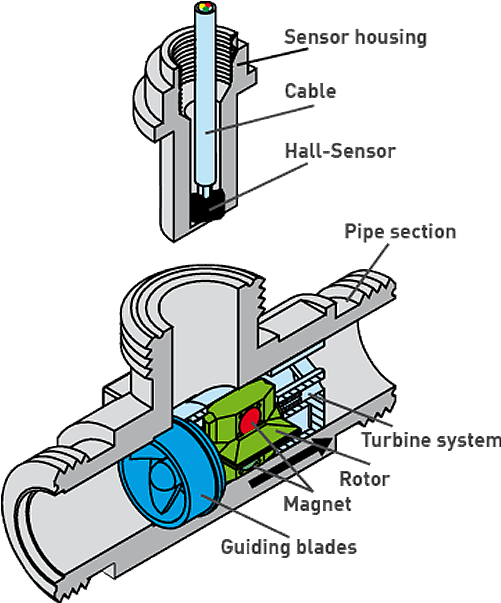
\includegraphics[width=0.7\textwidth]{pics/Turbinen_Durchfluss_Sensor.png}
    \caption{Schnittdarstellung des Turbinen-Durchflusssensors: Die einströmende Flüssigkeit versetzt den Rotor in Rotation, deren Frequenz vom Hall-Sensor erfasst und proportional zum Volumenstrom ausgewertet wird.}
    \label{fig:durchfluss_sensor_prinzip}
\end{figure}

\subsection{Temperatursensorik (PT1000)}
\label{subsec:pt1000}

Zur Erfassung der Kühlmitteltemperatur an kritischen Stellen des Kreislaufs -- insbesondere im Vor- und Rücklauf der Radiatoren -- werden zusätzliche PT1000-Widerstandsthermometer eingesetzt.

\begin{figure}[htbp]
    \centering
    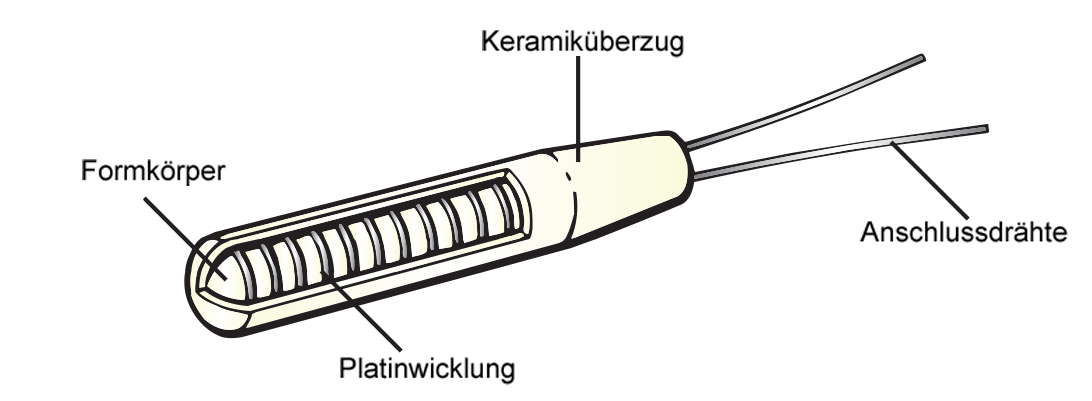
\includegraphics[width=0.6\textwidth]{pics/PT_100_Skizze.png}
    \caption{Schematischer Aufbau eines PT100-Widerstandsthermometers mit Platinwicklung und Keramikschutzmantel.}
    \label{fig:pt1000_aufbau}
\end{figure}

Das Messprinzip basiert auf dem positiven Temperaturkoeffizienten (PTC) von Platin: Mit steigender Temperatur erhöht sich der elektrische Widerstand der Platinwicklung nahezu linear. Ein PT1000 besitzt bei $0\,^\circ\text{C}$ einen Nennwiderstand von $1000\,\Omega$. Die Widerstandsänderung wird über eine Wheatstone-Messbrücke in der VCU ausgewertet und in einen kalibrierten Temperaturwert umgerechnet. Platin zeichnet sich dabei durch eine exzellente Langzeitstabilität aus, was wiederholte Messungen unter Wettbewerbsbedingungen zuverlässig reproduzierbar macht.

\subsection{Differenzdrucksensor (Piezoresistiv)}
\label{subsec:drucksensor}

Zur Bestimmung von Druckverlusten innerhalb des Kühlkreislaufs -- beispielsweise über dem Radiator -- werden piezoresistive Differenzdrucksensoren eingesetzt. Im Gegensatz zu Absolutdrucksensoren verfügen diese über zwei Druckanschlüsse ($P_1$ und $P_2$), sodass direkt die Druckdifferenz $\Delta p = P_1 - P_2$ gemessen wird.

\begin{figure}[htbp]
    \centering
    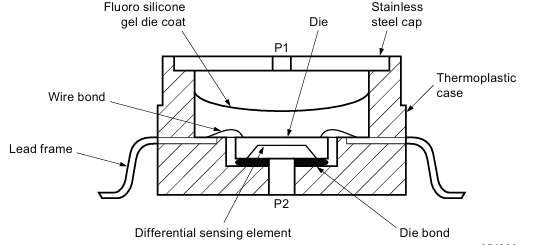
\includegraphics[width=0.7\textwidth]{pics/Piezo_Kristall_MTP.PNG}
    \caption{Interner Aufbau eines piezoresistiven Differenzdrucksensors: Die Druckdifferenz verformt eine Siliziummembran, deren Widerstandsänderung über eine Wheatstone-Brücke ausgewertet wird.}
    \label{fig:drucksensor_aufbau}
\end{figure}

Das Herzstück des Sensors bildet eine dünne Siliziummembran. Eine anliegende Druckdifferenz führt zu deren mechanischer Verformung, wodurch sich der elektrische Widerstand der aufgebrachten piezoresistiven Elemente ändert. Diese sind in einer Wheatstone-Messbrücke verschaltet, die die Dehnung in eine proportionale Ausgangsspannung umwandelt. Zum Schutz der empfindlichen Halbleiterstruktur vor dem Kühlmedium ist das Sensorelement mit einem chemisch inerten Silikon-Gel vergossen, das den hydraulischen Druck verlustfrei überträgt und die Elektronik gleichzeitig isoliert.

% -------------------------------------------------------
\section{Positionierung und Validierung der Sensorik}
\label{sec:validierung}

\subsection{Sensorik und Validierung}
\label{subsec:sensorik}

\subsubsection{Volumenstromsensor}

Der Volumenstromsensor dient dazu, im Stand bzw. im geschlossenen
Kühlkreislauf den Volumenstrom zu bestimmen. Anhand der bekannten
Pumpenkennlinie und der Stromaufnahme der Pumpe kann anschließend geprüft
werden, ob dieser Volumenstrom auch in anderen Betriebssituationen erreicht
wird. Treten Abweichungen auf, lassen sich deren Ursachen und Randbedingungen
eingrenzen.

\subsubsection{Temperatursensorik und Ausbaustrategie}

Die Temperatursensorik wurde im Verlauf der Arbeit entwickelt. Aufgrund der
geringen Verfügbarkeit der WPMD-Platinen konnte bisher nur ein Radpaket
ausgestattet werden. Ein Nachrüsten weiterer Sensoren ist vorgesehen.
Die erarbeitete Strategie gliedert sich in drei Stufen:

\begin{description}
    \item[Stufe 1] Vermessung eines Motors an einem Radpaket. Damit lässt sich
          die grundsätzliche Kühlmitteltemperatur validieren. Aus bekanntem
          Volumenstrom und Temperaturanstieg kann zudem ein Wärmestrom
          bestimmt werden. Wegen der thermischen Trägheit des Motors ist
          dies jedoch nur für quasistatische Fahrsituationen aussagekräftig.
    \item[Stufe 2] Ein Radpaketpaar, ein Inverterpaar und ein Radiatorpaar.
          Damit können alle Komponenten eines Kühlkreislaufs klassifiziert
          werden. Die ermittelten Kennwerte sind Grundlage für die in
          Abschnitt~\ref{TODO_Abschnitt} entwickelten Systemmodelle.
    \item[Stufe 3] Vollständige Vermessung. Alle vier Motoren erhalten ein
          Temperatursensorpaar, ebenso die Inverterkühlung sowie beide
          Radiatoren. Zusätzliche Sensoren erfassen die Lufttemperatur.
\end{description}

\subsubsection{Validierung der Sensorik}

\paragraph{Volumenstrom.} Der Sensor wurde durch Auffangen des Förderstroms
in einem Behälter überprüft. In $t = 60\,\mathrm{s}$ wurden
$V = 21\,\mathrm{l}$ gefördert. Daraus ergibt sich der Referenzvolumenstrom
\begin{equation}
    \dot{V}_\mathrm{ref} = \frac{V}{t}
    = \frac{21\,\mathrm{l}}{60\,\mathrm{s}}
    = 21\,\mathrm{l/min} = 0{,}35\,\mathrm{l/s}.
\end{equation}
Der Sensor zeigte $\dot{V}_\mathrm{Sensor} = 21{,}7\,\mathrm{l/min}$. Die
relative Abweichung beträgt
\begin{equation}
    e = \frac{\dot{V}_\mathrm{Sensor} - \dot{V}_\mathrm{ref}}{\dot{V}_\mathrm{ref}}
    = 3{,}33\,\%.
\end{equation}
Sie liegt innerhalb der Herstellertoleranz von $10\,\%$. Zusätzlich
wurde während des Versuchs eine Pumpenstromaufnahme von $3\,\mathrm{A}$
gemessen, die als Referenz für den weiteren Betrieb dient. Die Unsicherheit
der Referenzmessung aus Zeitnahme und Volumenablesung beträgt $2{,}5\,\%$.

\paragraph{Temperatur: Versuchsdurchführung.} Alle PT100-Sensoren wurden
gleichzeitig in siedendes Wasser getaucht. Nach Einstellen eines stationären
Plateaus wurde über $t = 150\,\mathrm{s}$ per Handnotiz aufgezeichnet. Die Referenztemperatur folgt aus dem
Luftdruck am Messtag ($p = 964\,\mathrm{hPa}$) zu
$T_\mathrm{ref} = 98{,}61\,^\circ\mathrm{C}$.

\paragraph{Temperatur: Auswertung.} Je Sensor $i$ wird der Mittelwert
$\bar{T}_i$ im Plateau gebildet. Die Abweichung zur Referenz ist
$\Delta T_i = \bar{T}_i - T_\mathrm{ref}$. Als Streuung zwischen den
Sensoren dient die Standardabweichung der $\bar{T}_i$.

\begin{table}[htbp]
    \centering
    \caption{Ergebnis des Siedetests der PT100-Sensoren}
    \label{tab:pt100_siedetest}
    \begin{tabular}{lrrr}
        \hline
        Sensor & $\bar{T}_i$ in $^\circ\mathrm{C}$ & $\Delta T_i$ in $\mathrm{K}$ & $s_i$ in $\mathrm{K}$ \\
        \hline
        Sensor 1 & $98{,}52$ & $-0{,}09$ & $0{,}03$ \\
        Sensor 2 & $98{,}78$ & $0{,}17$  & $0{,}05$ \\
        Sensor 3 & $98{,}47$ & $-0{,}14$ & $0{,}04$ \\
        Sensor 4 & $98{,}66$ & $0{,}05$  & $0{,}04$ \\
        Sensor 5 & $98{,}81$ & $0{,}20$  & $0{,}03$ \\
        \hline
    \end{tabular}
\end{table}

\paragraph{Temperatur: Bewertung.} Die maximale Abweichung beträgt
$0{,}20\,\mathrm{K}$, die Streuung zwischen den Sensoren
$0{,}15\,\mathrm{K}$. Zum Vergleich: Die Toleranz nach DIN EN 60751 beträgt
bei $100\,^\circ\mathrm{C}$ für Klasse~A $0{,}35\,\mathrm{K}$ und für
Klasse~B $0{,}8\,\mathrm{K}$. Der Test erfolgte als Einpunktprüfung bei etwa
$100\,^\circ\mathrm{C}$, eine Aussage über den gesamten Betriebsbereich ist
daraus nicht ableitbar.

\paragraph{Temperatur: Zeitkonstante.} Zur Bestimmung der Zeitkonstante
$\tau$ wird zunächst vor dem Versuch die relevante Schwellentemperatur
berechnet. Dazu werden der Anfangswert $T_0$ (Sensor in Raumluft) und der
Endwert $T_\infty$ (gerührtes siedendes Wasser) herangezogen. Für ein
Verzögerungsglied 1.~Ordnung
\begin{equation}
    T(t) = T_\infty - (T_\infty - T_0)\,e^{-t/\tau}
\end{equation}
ist $\tau$ genau dann verstrichen, wenn der Sensor $63{,}2\,\%$ des
Temperatursprungs durchlaufen hat:
\begin{equation}
    T_\tau = T_0 + 0{,}632\,(T_\infty - T_0)
    = 22{,}4\,^\circ\mathrm{C} + 0{,}632 \cdot 76{,}2\,\mathrm{K}
    = 70{,}6\,^\circ\mathrm{C}.
\end{equation}
Anschließend wird der Sensor aus Raumluft schnell in das gerührte
siedende Wasser getaucht und mit $5\,\mathrm{Hz}$ aufgezeichnet. Die
Zeitkonstante $\tau$ ist die Zeit zwischen dem Eintauchen (Signal verlässt
$T_0$) und dem erstmaligen Erreichen von $T_\tau$. Bei $5\,\mathrm{Hz}$
beträgt die Zeitauflösung $0{,}2\,\mathrm{s}$.

\begin{table}[htbp]
    \centering
    \caption{Zeitkonstanten der PT100-Sensoren im gerührten Wasserbad}
    \label{tab:pt100_tau}
    \begin{tabular}{lrrr}
        \hline
        Sensor & $t_{63}$ in $\mathrm{s}$ & $\tau_\mathrm{Fit}$ in $\mathrm{s}$ & $t_{90}$ in $\mathrm{s}$ \\
        \hline
        Sensor 1 & $3{,}4$ & $3{,}3$ & $7{,}6$ \\
        Sensor 2 & $3{,}6$ & $3{,}6$ & $8{,}3$ \\
        Sensor 3 & $3{,}0$ & $2{,}9$ & $6{,}7$ \\
        Sensor 4 & $3{,}1$ & $3{,}1$ & $7{,}1$ \\
        Sensor 5 & $4{,}2$ & $4{,}1$ & $9{,}4$ \\
        \hline
    \end{tabular}
\end{table}

\paragraph{Temperatur: Bewertung der Zeitkonstante.} Die Zeitkonstanten
liegen zwischen $2{,}9\,\mathrm{s}$ und $4{,}1\,\mathrm{s}$. Bei einer
Temperaturrampe $\mathrm{d}T/\mathrm{d}t$ zeigt der Sensor einen
Schleppfehler von $\Delta T = \tau \cdot \mathrm{d}T/\mathrm{d}t$, bei
$0{,}5\,\mathrm{K/s}$ und $\tau = 3{,}6\,\mathrm{s}$ also
$1{,}8\,\mathrm{K}$. Die Werte gelten für die Umströmung im Wasserbad
und können im Kühlkreis mit anderer Strömungsgeschwindigkeit abweichen.

\section{Ausarbeitung eines Testplanes}
\label{sec:Testplanung}

% TODO: Abschnitt nach Abschluss der Messungen ausformulieren.
% Geplante Messprogramme:
%
% Motoren:
%   - Thermische Masse (Gewichtsmessung + Datenblattwerte)
%   - Wärmeübergangskoeffizient (Abkühlversuch mit temperiertem Wasser)
%
% Inverter:
%   - Thermische Masse (Gewichtsmessung + Datenblattwerte)
%   - Wärmeübergangskoeffizient
%
% Pumpen:
%   - Volumenstrom-Kennlinie in Abhängigkeit des PWM-Signals (Testaufbau)
%
% Radiatoren:
%   - Wärmeübertragungskoeffizient (temperiertes Wasser, Vor-/Rücklauftemperatur,
%     Volumenstrom; ggf. Windkanal OTH)
%
% Lüfter:
%   - Luftvolumenstrom im Stand (Lüfter aktiv)
%   - Luftvolumenstrom unter der Fahrt
%   - Wärmeübergangskoeffizient unter Fahrtwind